\documentclass[12pt]{beamer}\usepackage[]{graphicx}\usepackage[]{color}
%% maxwidth is the original width if it is less than linewidth
%% otherwise use linewidth (to make sure the graphics do not exceed the margin)
\makeatletter
\def\maxwidth{ %
  \ifdim\Gin@nat@width>\linewidth
    \linewidth
  \else
    \Gin@nat@width
  \fi
}
\makeatother

\definecolor{fgcolor}{rgb}{0.345, 0.345, 0.345}
\newcommand{\hlnum}[1]{\textcolor[rgb]{0.686,0.059,0.569}{#1}}%
\newcommand{\hlstr}[1]{\textcolor[rgb]{0.192,0.494,0.8}{#1}}%
\newcommand{\hlcom}[1]{\textcolor[rgb]{0.678,0.584,0.686}{\textit{#1}}}%
\newcommand{\hlopt}[1]{\textcolor[rgb]{0,0,0}{#1}}%
\newcommand{\hlstd}[1]{\textcolor[rgb]{0.345,0.345,0.345}{#1}}%
\newcommand{\hlkwa}[1]{\textcolor[rgb]{0.161,0.373,0.58}{\textbf{#1}}}%
\newcommand{\hlkwb}[1]{\textcolor[rgb]{0.69,0.353,0.396}{#1}}%
\newcommand{\hlkwc}[1]{\textcolor[rgb]{0.333,0.667,0.333}{#1}}%
\newcommand{\hlkwd}[1]{\textcolor[rgb]{0.737,0.353,0.396}{\textbf{#1}}}%

\usepackage{framed}
\makeatletter
\newenvironment{kframe}{%
 \def\at@end@of@kframe{}%
 \ifinner\ifhmode%
  \def\at@end@of@kframe{\end{minipage}}%
  \begin{minipage}{\columnwidth}%
 \fi\fi%
 \def\FrameCommand##1{\hskip\@totalleftmargin \hskip-\fboxsep
 \colorbox{shadecolor}{##1}\hskip-\fboxsep
     % There is no \\@totalrightmargin, so:
     \hskip-\linewidth \hskip-\@totalleftmargin \hskip\columnwidth}%
 \MakeFramed {\advance\hsize-\width
   \@totalleftmargin\z@ \linewidth\hsize
   \@setminipage}}%
 {\par\unskip\endMakeFramed%
 \at@end@of@kframe}
\makeatother

\definecolor{shadecolor}{rgb}{.97, .97, .97}
\definecolor{messagecolor}{rgb}{0, 0, 0}
\definecolor{warningcolor}{rgb}{1, 0, 1}
\definecolor{errorcolor}{rgb}{1, 0, 0}
\newenvironment{knitrout}{}{} % an empty environment to be redefined in TeX

\usepackage{alltt}
\usepackage{graphicx}
\usepackage{tikz}
\setbeameroption{hide notes}
\setbeamertemplate{note page}[plain]
\usepackage{listings}

% get rid of junk
\usetheme{default}
\usefonttheme[onlymath]{serif}
\beamertemplatenavigationsymbolsempty
\hypersetup{pdfpagemode=UseNone} % don't show bookmarks on initial view

% named colors
\definecolor{offwhite}{RGB}{255,250,240}
\definecolor{gray}{RGB}{155,155,155}

\ifx\notescolors\undefined % slides

  \definecolor{foreground}{RGB}{80,80,80}
  \definecolor{background}{RGB}{255,255,255}
  \definecolor{title}{RGB}{255,199,0}
  \definecolor{subtitle}{RGB}{89,132,212}
  \definecolor{hilit}{RGB}{248,117,79}
  \definecolor{vhilit}{RGB}{255,111,207}
  \definecolor{lolit}{RGB}{200,200,200}
  \definecolor{lit}{RGB}{255,199,0}
  \definecolor{mdlit}{RGB}{89,132,212}
  \definecolor{link}{RGB}{248,117,79}

\else % notes
  \definecolor{background}{RGB}{255,255,255}
  \definecolor{foreground}{RGB}{24,24,24}
  \definecolor{title}{RGB}{27,94,134}
  \definecolor{subtitle}{RGB}{22,175,124}
  \definecolor{hilit}{RGB}{122,0,128}
  \definecolor{vhilit}{RGB}{255,0,128}
  \definecolor{lolit}{RGB}{95,95,95}
\fi
\definecolor{nhilit}{RGB}{128,0,128}  % hilit color in notes
\definecolor{nvhilit}{RGB}{255,0,128} % vhilit for notes

\newcommand{\hilit}{\color{hilit}}
\newcommand{\vhilit}{\color{vhilit}}
\newcommand{\nhilit}{\color{nhilit}}
\newcommand{\nvhilit}{\color{nvhilit}}
\newcommand{\lit}{\color{lit}}
\newcommand{\mdlit}{\color{mdlit}}
\newcommand{\lolit}{\color{lolit}}

% use those colors
\setbeamercolor{titlelike}{fg=title}
\setbeamercolor{subtitle}{fg=subtitle}
\setbeamercolor{frametitle}{fg=gray}
\setbeamercolor{structure}{fg=subtitle}
\setbeamercolor{institute}{fg=lolit}
\setbeamercolor{normal text}{fg=foreground,bg=background}
%\setbeamercolor{item}{fg=foreground} % color of bullets
%\setbeamercolor{subitem}{fg=hilit}
%\setbeamercolor{itemize/enumerate subbody}{fg=lolit}
\setbeamertemplate{itemize subitem}{{\textendash}}
\setbeamerfont{itemize/enumerate subbody}{size=\footnotesize}
\setbeamerfont{itemize/enumerate subitem}{size=\footnotesize}

% center title of slides
\setbeamertemplate{blocks}[rounded]
\setbeamertemplate{frametitle}[default][center]
% margins
\setbeamersize{text margin left=25pt,text margin right=25pt}

% page number
\setbeamertemplate{footline}{%
    \raisebox{5pt}{\makebox[\paperwidth]{\hfill\makebox[20pt]{\lolit
          \scriptsize\insertframenumber}}}\hspace*{5pt}}

% add a bit of space at the top of the notes page
\addtobeamertemplate{note page}{\setlength{\parskip}{12pt}}

% default link color
\hypersetup{colorlinks, urlcolor={link}}

\ifx\notescolors\undefined % slides
  % set up listing environment
  \lstset{language=bash,
          basicstyle=\ttfamily\scriptsize,
          frame=single,
          commentstyle=,
          backgroundcolor=\color{darkgray},
          showspaces=false,
          showstringspaces=false
          }
\else % notes
  \lstset{language=bash,
          basicstyle=\ttfamily\scriptsize,
          frame=single,
          commentstyle=,
          backgroundcolor=\color{offwhite},
          showspaces=false,
          showstringspaces=false
          }
\fi

% a few macros
\newcommand{\code}[1]{\texttt{#1}}
\newcommand{\hicode}[1]{{\hilit \texttt{#1}}}
\newcommand{\bb}[1]{\begin{block}{#1}}
\newcommand{\eb}{\end{block}}
\newcommand{\bi}{\begin{itemize}}
%\newcommand{\bbi}{\vspace{24pt} \begin{itemize} \itemsep8pt}
\newcommand{\bbi}{\vspace{4pt} \begin{itemize} \itemsep8pt}
\newcommand{\ei}{\end{itemize}}
\newcommand{\bv}{\begin{verbatim}}
\newcommand{\ev}{\end{verbatim}}
\newcommand{\ig}{\includegraphics}
\newcommand{\subt}[1]{{\footnotesize \color{subtitle} {#1}}}
\newcommand{\ttsm}{\tt \small}
\newcommand{\ttfn}{\tt \footnotesize}
\newcommand{\figh}[2]{\centerline{\includegraphics[height=#2\textheight]{#1}}}
\newcommand{\figw}[2]{\centerline{\includegraphics[width=#2\textwidth]{#1}}}



%------------------------------------------------
% end of header
%------------------------------------------------

\title{Handling Missing Values}
\subtitle{STAT 133}
\author{\href{http://www.gastonsanchez.com}{Gaston Sanchez}}
\institute{Department of Statistics, UC{\textendash}Berkeley}
\date{\href{http://www.gastonsanchez.com}{\tt \scriptsize \color{foreground} gastonsanchez.com}
\\[-4pt]
\href{http://github.com/gastonstat/stat133}{\tt \scriptsize \color{foreground} github.com/gastonstat/stat133}
\\[-4pt]
{\scriptsize Course web: \href{http://www.gastonsanchez.com/stat133}{\tt gastonsanchez.com/stat133}}
}
\IfFileExists{upquote.sty}{\usepackage{upquote}}{}
\begin{document}


{
  \setbeamertemplate{footline}{} % no page number here
  \frame{
    \titlepage
  } 
}

%------------------------------------------------

\begin{frame}
\begin{center}
\Huge{\hilit{Missing Values}}
\end{center}
\end{frame}

%------------------------------------------------

\begin{frame}[fragile]
\frametitle{Introduction}

\bb{Missing Values are very common}
\bbi
  \item ``no answer'' in a questionnaire / survey
  \item data that are lost or destroyed
  \item machines that fail
  \item experiments/samples that are lost
  \item things not working
\ei
\eb

\end{frame}

%------------------------------------------------

\begin{frame}
\frametitle{Introduction}

{\Large The best thing to do about missing values is not to have any}

\bigskip
Gertrude Cox

\end{frame}

%------------------------------------------------

\begin{frame}
\frametitle{Missing Values}

\bb{Missing Values in R}
\bbi
  \item Missing values in R are denoted with {\hilit \code{NA}}
  \item \code{NA} stands for \textbf{Not Available}
  \item \code{NA} is actually a \textbf{logical} value
  \item Do not confuse \code{NA} with \code{"NA"} (character)
  \item Do not confuse \code{NA} with \code{NaN} (not a number)
\ei
\eb

\end{frame}

%------------------------------------------------

\begin{frame}[fragile]
\frametitle{Missing Values Functions in R}

\begin{knitrout}\footnotesize
\definecolor{shadecolor}{rgb}{0.969, 0.969, 0.969}\color{fgcolor}\begin{kframe}
\begin{alltt}
\hlcom{# NA is a logical value}
\hlkwd{is.logical}\hlstd{(}\hlnum{NA}\hlstd{)}
\end{alltt}
\begin{verbatim}
## [1] TRUE
\end{verbatim}
\begin{alltt}
\hlcom{# NA is not the same as NaN}
\hlkwd{identical}\hlstd{(}\hlnum{NA}\hlstd{,} \hlnum{NaN}\hlstd{)}
\end{alltt}
\begin{verbatim}
## [1] FALSE
\end{verbatim}
\begin{alltt}
\hlcom{# NA is not the same as "NA"}
\hlkwd{identical}\hlstd{(}\hlnum{NA}\hlstd{,} \hlstr{"NA"}\hlstd{)}
\end{alltt}
\begin{verbatim}
## [1] FALSE
\end{verbatim}
\end{kframe}
\end{knitrout}

\end{frame}

%------------------------------------------------

\begin{frame}[fragile]
\frametitle{Function \code{is.na()}}

\bi
  \item {\hilit \code{is.na()}} indicates which elements are missing
  \item \code{is.na()} is a generic function (i.e. can be used for vectors, factors, matrices, etc)
\ei

\begin{knitrout}\footnotesize
\definecolor{shadecolor}{rgb}{0.969, 0.969, 0.969}\color{fgcolor}\begin{kframe}
\begin{alltt}
\hlstd{x} \hlkwb{<-} \hlkwd{c}\hlstd{(}\hlnum{1}\hlstd{,} \hlnum{2}\hlstd{,} \hlnum{3}\hlstd{,} \hlnum{NA}\hlstd{,} \hlnum{5}\hlstd{)}
\hlstd{x}
\end{alltt}
\begin{verbatim}
## [1]  1  2  3 NA  5
\end{verbatim}
\begin{alltt}
\hlkwd{is.na}\hlstd{(x)}
\end{alltt}
\begin{verbatim}
## [1] FALSE FALSE FALSE  TRUE FALSE
\end{verbatim}
\end{kframe}
\end{knitrout}

\end{frame}

%------------------------------------------------

\begin{frame}[fragile]
\frametitle{Function \code{is.na()}}

\code{is.na()} on a factor
\begin{knitrout}\footnotesize
\definecolor{shadecolor}{rgb}{0.969, 0.969, 0.969}\color{fgcolor}\begin{kframe}
\begin{alltt}
\hlstd{g} \hlkwb{<-} \hlkwd{factor}\hlstd{(}\hlkwd{c}\hlstd{(letters[}\hlkwd{rep}\hlstd{(}\hlnum{1}\hlopt{:}\hlnum{3}\hlstd{,} \hlnum{2}\hlstd{)],} \hlnum{NA}\hlstd{))}
\hlstd{g}
\end{alltt}
\begin{verbatim}
## [1] a    b    c    a    b    c    <NA>
## Levels: a b c
\end{verbatim}
\begin{alltt}
\hlkwd{is.na}\hlstd{(g)}
\end{alltt}
\begin{verbatim}
## [1] FALSE FALSE FALSE FALSE FALSE FALSE  TRUE
\end{verbatim}
\end{kframe}
\end{knitrout}

{\footnotesize Notice how missing values are denoted in factors}

\end{frame}

%------------------------------------------------

\begin{frame}[fragile]
\frametitle{Function \code{is.na()}}

\code{is.na()} on a matrix
\begin{knitrout}\footnotesize
\definecolor{shadecolor}{rgb}{0.969, 0.969, 0.969}\color{fgcolor}\begin{kframe}
\begin{alltt}
\hlstd{m} \hlkwb{<-} \hlkwd{matrix}\hlstd{(}\hlkwd{c}\hlstd{(}\hlnum{1}\hlopt{:}\hlnum{4}\hlstd{,} \hlnum{NA}\hlstd{,} \hlnum{6}\hlopt{:}\hlnum{9}\hlstd{,} \hlnum{NA}\hlstd{),} \hlnum{2}\hlstd{)}
\hlstd{m}
\end{alltt}
\begin{verbatim}
##      [,1] [,2] [,3] [,4] [,5]
## [1,]    1    3   NA    7    9
## [2,]    2    4    6    8   NA
\end{verbatim}
\begin{alltt}
\hlkwd{is.na}\hlstd{(m)}
\end{alltt}
\begin{verbatim}
##       [,1]  [,2]  [,3]  [,4]  [,5]
## [1,] FALSE FALSE  TRUE FALSE FALSE
## [2,] FALSE FALSE FALSE FALSE  TRUE
\end{verbatim}
\end{kframe}
\end{knitrout}

\end{frame}

%------------------------------------------------

\begin{frame}[fragile]
\frametitle{Function \code{is.na()}}

\code{is.na()} on a data.frame
\begin{knitrout}\footnotesize
\definecolor{shadecolor}{rgb}{0.969, 0.969, 0.969}\color{fgcolor}\begin{kframe}
\begin{alltt}
\hlstd{d} \hlkwb{<-} \hlkwd{data.frame}\hlstd{(m)}
\hlstd{d}
\end{alltt}
\begin{verbatim}
##   X1 X2 X3 X4 X5
## 1  1  3 NA  7  9
## 2  2  4  6  8 NA
\end{verbatim}
\begin{alltt}
\hlkwd{is.na}\hlstd{(d)}
\end{alltt}
\begin{verbatim}
##         X1    X2    X3    X4    X5
## [1,] FALSE FALSE  TRUE FALSE FALSE
## [2,] FALSE FALSE FALSE FALSE  TRUE
\end{verbatim}
\end{kframe}
\end{knitrout}

\end{frame}

%------------------------------------------------

\begin{frame}[fragile]
\frametitle{Function \code{is.na()}}

If you're reading a data table with missing values codified differently from \code{NA}, you can specify the parameter {\hilit \code{na.strings}}

\begin{knitrout}\scriptsize
\definecolor{shadecolor}{rgb}{0.969, 0.969, 0.969}\color{fgcolor}\begin{kframe}
\begin{alltt}
\hlstd{url} \hlkwb{<-} \hlstr{"http://www.esapubs.org/archive/ecol/E084/094/MOMv3.3.txt"}

\hlstd{df} \hlkwb{<-} \hlkwd{read.table}\hlstd{(}\hlkwc{file} \hlstd{= url,} \hlkwc{header} \hlstd{=} \hlnum{FALSE}\hlstd{,}
                 \hlkwc{sep} \hlstd{=} \hlstr{"\textbackslash{}t"}\hlstd{,} \hlkwc{na.strings} \hlstd{=} \hlopt{-}\hlnum{999}\hlstd{)}
\end{alltt}
\end{kframe}
\end{knitrout}

\end{frame}

%------------------------------------------------

\begin{frame}
\begin{center}
\Huge{\hilit{Computing with \code{NA}s}}
\end{center}
\end{frame}

%------------------------------------------------

\begin{frame}[fragile]
\frametitle{Computing with \code{NA}'s}

Numerical computations using \code{NA} will normally result in \code{NA}
\begin{knitrout}\footnotesize
\definecolor{shadecolor}{rgb}{0.969, 0.969, 0.969}\color{fgcolor}\begin{kframe}
\begin{alltt}
\hlnum{2} \hlopt{+} \hlnum{NA}
\end{alltt}
\begin{verbatim}
## [1] NA
\end{verbatim}
\begin{alltt}
\hlstd{x} \hlkwb{<-} \hlkwd{c}\hlstd{(}\hlnum{1}\hlstd{,} \hlnum{2}\hlstd{,} \hlnum{3}\hlstd{,} \hlnum{NA}\hlstd{,} \hlnum{5}\hlstd{)}
\hlstd{x} \hlopt{+} \hlnum{1}
\end{alltt}
\begin{verbatim}
## [1]  2  3  4 NA  6
\end{verbatim}
\end{kframe}
\end{knitrout}

\end{frame}

%------------------------------------------------

\begin{frame}[fragile]
\frametitle{Computing with \code{NA}'s}

\begin{knitrout}\footnotesize
\definecolor{shadecolor}{rgb}{0.969, 0.969, 0.969}\color{fgcolor}\begin{kframe}
\begin{alltt}
\hlkwd{sqrt}\hlstd{(x)}
\end{alltt}
\begin{verbatim}
## [1] 1.000000 1.414214 1.732051       NA 2.236068
\end{verbatim}
\begin{alltt}
\hlkwd{mean}\hlstd{(x)}
\end{alltt}
\begin{verbatim}
## [1] NA
\end{verbatim}
\begin{alltt}
\hlkwd{max}\hlstd{(x)}
\end{alltt}
\begin{verbatim}
## [1] NA
\end{verbatim}
\end{kframe}
\end{knitrout}

\end{frame}

%------------------------------------------------

\begin{frame}
\frametitle{Argument \code{na.rm}}

Most arithmetic/trigonometric/summarizing functions provide the argument {\hilit \code{na.rm = TRUE}} that removes missing values before performing the computation:
\bi
  \item \code{mean(x, na.rm = TRUE)}
  \item \code{sd(x, na.rm = TRUE)}
  \item \code{var(x, na.rm = TRUE)}
  \item \code{min(x, na.rm = TRUE)}
  \item \code{max(x, na.rm = TRUE)}
  \item \code{sum(x, na.rm = TRUE)}
  \item \textit{etc}
\ei

\end{frame}

%------------------------------------------------

\begin{frame}[fragile]
\frametitle{Argument \code{na.rm}}

\begin{knitrout}\footnotesize
\definecolor{shadecolor}{rgb}{0.969, 0.969, 0.969}\color{fgcolor}\begin{kframe}
\begin{alltt}
\hlstd{x} \hlkwb{<-} \hlkwd{c}\hlstd{(}\hlnum{1}\hlstd{,} \hlnum{2}\hlstd{,} \hlnum{3}\hlstd{,} \hlnum{NA}\hlstd{,} \hlnum{5}\hlstd{)}

\hlkwd{mean}\hlstd{(x,} \hlkwc{na.rm} \hlstd{=} \hlnum{TRUE}\hlstd{)}
\end{alltt}
\begin{verbatim}
## [1] 2.75
\end{verbatim}
\begin{alltt}
\hlkwd{sd}\hlstd{(x,} \hlkwc{na.rm} \hlstd{=} \hlnum{TRUE}\hlstd{)}
\end{alltt}
\begin{verbatim}
## [1] 1.707825
\end{verbatim}
\begin{alltt}
\hlkwd{median}\hlstd{(x,} \hlkwc{na.rm} \hlstd{=} \hlnum{TRUE}\hlstd{)}
\end{alltt}
\begin{verbatim}
## [1] 2.5
\end{verbatim}
\end{kframe}
\end{knitrout}

\end{frame}

%------------------------------------------------

\begin{frame}[fragile]
\frametitle{Argument \code{na.rm}}

\begin{knitrout}\footnotesize
\definecolor{shadecolor}{rgb}{0.969, 0.969, 0.969}\color{fgcolor}\begin{kframe}
\begin{alltt}
\hlstd{x} \hlkwb{<-} \hlkwd{c}\hlstd{(}\hlnum{1}\hlstd{,} \hlnum{2}\hlstd{,} \hlnum{3}\hlstd{,} \hlnum{NA}\hlstd{,} \hlnum{5}\hlstd{)}

\hlstd{y} \hlkwb{<-} \hlkwd{c}\hlstd{(}\hlnum{2}\hlstd{,} \hlnum{4}\hlstd{,} \hlnum{7}\hlstd{,} \hlnum{9}\hlstd{,} \hlnum{11}\hlstd{)}

\hlkwd{var}\hlstd{(x, y,} \hlkwc{na.rm} \hlstd{=} \hlnum{TRUE}\hlstd{)}
\end{alltt}
\begin{verbatim}
## [1] 6.666667
\end{verbatim}
\end{kframe}
\end{knitrout}

\end{frame}

%------------------------------------------------

\begin{frame}[fragile]
\frametitle{Correlations with \code{NA}}

\begin{knitrout}\footnotesize
\definecolor{shadecolor}{rgb}{0.969, 0.969, 0.969}\color{fgcolor}\begin{kframe}
\begin{alltt}
\hlcom{# default correlation}
\hlkwd{cor}\hlstd{(x, y)}
\end{alltt}
\begin{verbatim}
## [1] NA
\end{verbatim}
\begin{alltt}
\hlcom{# argument 'use'}
\hlkwd{cor}\hlstd{(x, y,} \hlkwc{use} \hlstd{=} \hlstr{'complete.obs'}\hlstd{)}
\end{alltt}
\begin{verbatim}
## [1] 0.9968896
\end{verbatim}
\end{kframe}
\end{knitrout}

\end{frame}

%------------------------------------------------

\begin{frame}
\begin{center}
\Huge{\hilit{\code{NA} Actions}}
\end{center}
\end{frame}

%------------------------------------------------

\begin{frame}
\frametitle{Argument \code{na.rm}}

Additional functions for handling missing values:
\bi
  \item \code{anyNA()}
  \item \code{na.omit()}
  \item \code{complete.cases()}
  \item \code{na.fail()}
  \item \code{na.exclude()}
  \item \code{na.pass()}
\ei

\end{frame}

%------------------------------------------------

\begin{frame}[fragile]
\frametitle{Checking for missing values}

A common operation is to check for the presence of missing values in a given object:
\begin{knitrout}\footnotesize
\definecolor{shadecolor}{rgb}{0.969, 0.969, 0.969}\color{fgcolor}\begin{kframe}
\begin{alltt}
\hlstd{x} \hlkwb{<-} \hlkwd{c}\hlstd{(}\hlnum{1}\hlstd{,} \hlnum{2}\hlstd{,} \hlnum{3}\hlstd{,} \hlnum{NA}\hlstd{,} \hlnum{5}\hlstd{)}

\hlkwd{any}\hlstd{(}\hlkwd{is.na}\hlstd{(x))}
\end{alltt}
\begin{verbatim}
## [1] TRUE
\end{verbatim}
\begin{alltt}
\hlcom{# alternatively}
\hlkwd{anyNA}\hlstd{(x)}
\end{alltt}
\begin{verbatim}
## [1] TRUE
\end{verbatim}
\end{kframe}
\end{knitrout}

\end{frame}

%------------------------------------------------

\begin{frame}[fragile]
\frametitle{Checking for missing values}

Another common operation is to calculate the number of missing values:
\begin{knitrout}\footnotesize
\definecolor{shadecolor}{rgb}{0.969, 0.969, 0.969}\color{fgcolor}\begin{kframe}
\begin{alltt}
\hlstd{y} \hlkwb{<-} \hlkwd{c}\hlstd{(}\hlnum{1}\hlstd{,} \hlnum{2}\hlstd{,} \hlnum{3}\hlstd{,} \hlnum{NA}\hlstd{,} \hlnum{5}\hlstd{,} \hlnum{NA}\hlstd{)}

\hlcom{# how many NA's}
\hlkwd{sum}\hlstd{(}\hlkwd{is.na}\hlstd{(y))}
\end{alltt}
\begin{verbatim}
## [1] 2
\end{verbatim}
\end{kframe}
\end{knitrout}

\end{frame}

%------------------------------------------------

\begin{frame}[fragile]
\frametitle{Excluding missing values}

Sometimes we want to ``remove'' missing values from a vector or factor:
\begin{knitrout}\footnotesize
\definecolor{shadecolor}{rgb}{0.969, 0.969, 0.969}\color{fgcolor}\begin{kframe}
\begin{alltt}
\hlstd{x} \hlkwb{<-} \hlkwd{c}\hlstd{(}\hlnum{1}\hlstd{,} \hlnum{2}\hlstd{,} \hlnum{3}\hlstd{,} \hlnum{NA}\hlstd{,} \hlnum{5}\hlstd{,} \hlnum{NA}\hlstd{)}

\hlcom{# excluding NA's}
\hlstd{x[}\hlopt{!}\hlkwd{is.na}\hlstd{(x)]}
\end{alltt}
\begin{verbatim}
## [1] 1 2 3 5
\end{verbatim}
\end{kframe}
\end{knitrout}

\end{frame}

%------------------------------------------------

\begin{frame}[fragile]
\frametitle{Excluding missing values}

Another way to ``remove'' missing values from a vector or factor is with {\hilit \code{na.omit()}}
\begin{knitrout}\footnotesize
\definecolor{shadecolor}{rgb}{0.969, 0.969, 0.969}\color{fgcolor}\begin{kframe}
\begin{alltt}
\hlstd{x} \hlkwb{<-} \hlkwd{c}\hlstd{(}\hlnum{1}\hlstd{,} \hlnum{2}\hlstd{,} \hlnum{3}\hlstd{,} \hlnum{NA}\hlstd{,} \hlnum{5}\hlstd{,} \hlnum{NA}\hlstd{)}

\hlcom{# removing NA's}
\hlkwd{na.omit}\hlstd{(x)}
\end{alltt}
\begin{verbatim}
## [1] 1 2 3 5
## attr(,"na.action")
## [1] 4 6
## attr(,"class")
## [1] "omit"
\end{verbatim}
\end{kframe}
\end{knitrout}

\end{frame}

%------------------------------------------------

\begin{frame}[fragile]
\frametitle{Excluding missing values}

There's also the {\hilit \code{na.exclude()}} function that we can use to ``remove'' missing values
\begin{knitrout}\footnotesize
\definecolor{shadecolor}{rgb}{0.969, 0.969, 0.969}\color{fgcolor}\begin{kframe}
\begin{alltt}
\hlstd{x} \hlkwb{<-} \hlkwd{c}\hlstd{(}\hlnum{1}\hlstd{,} \hlnum{2}\hlstd{,} \hlnum{3}\hlstd{,} \hlnum{NA}\hlstd{,} \hlnum{5}\hlstd{,} \hlnum{NA}\hlstd{)}

\hlcom{# removing NA's}
\hlkwd{na.exclude}\hlstd{(x)}
\end{alltt}
\begin{verbatim}
## [1] 1 2 3 5
## attr(,"na.action")
## [1] 4 6
## attr(,"class")
## [1] "exclude"
\end{verbatim}
\end{kframe}
\end{knitrout}

\end{frame}

%------------------------------------------------

\begin{frame}[fragile]
\frametitle{Excluding rows with missing values}

Applying {\hilit \code{na.omit()}} on matrices or data frames will exclude the rows containing any missing value
\begin{knitrout}\footnotesize
\definecolor{shadecolor}{rgb}{0.969, 0.969, 0.969}\color{fgcolor}\begin{kframe}
\begin{alltt}
\hlstd{DF} \hlkwb{<-} \hlkwd{data.frame}\hlstd{(}\hlkwc{x} \hlstd{=} \hlkwd{c}\hlstd{(}\hlnum{1}\hlstd{,} \hlnum{2}\hlstd{,} \hlnum{3}\hlstd{),} \hlkwc{y} \hlstd{=} \hlkwd{c}\hlstd{(}\hlnum{0}\hlstd{,} \hlnum{10}\hlstd{,} \hlnum{NA}\hlstd{))}
\hlstd{DF}
\end{alltt}
\begin{verbatim}
##   x  y
## 1 1  0
## 2 2 10
## 3 3 NA
\end{verbatim}
\begin{alltt}
\hlcom{# how many NA's}
\hlkwd{na.omit}\hlstd{(DF)}
\end{alltt}
\begin{verbatim}
##   x  y
## 1 1  0
## 2 2 10
\end{verbatim}
\end{kframe}
\end{knitrout}

\end{frame}

%------------------------------------------------

\begin{frame}[fragile]
\frametitle{Function \code{complete.cases()}}

Likewise, we can use {\hilit \code{complete.cases()}} to get a logical vector with the position of those rows having complete data:
\begin{knitrout}\footnotesize
\definecolor{shadecolor}{rgb}{0.969, 0.969, 0.969}\color{fgcolor}\begin{kframe}
\begin{alltt}
\hlstd{DF} \hlkwb{<-} \hlkwd{data.frame}\hlstd{(}\hlkwc{x} \hlstd{=} \hlkwd{c}\hlstd{(}\hlnum{1}\hlstd{,} \hlnum{2}\hlstd{,} \hlnum{3}\hlstd{),} \hlkwc{y} \hlstd{=} \hlkwd{c}\hlstd{(}\hlnum{0}\hlstd{,} \hlnum{10}\hlstd{,} \hlnum{NA}\hlstd{))}

\hlcom{# how many NA's}
\hlkwd{complete.cases}\hlstd{(DF)}
\end{alltt}
\begin{verbatim}
## [1]  TRUE  TRUE FALSE
\end{verbatim}
\end{kframe}
\end{knitrout}

\end{frame}

%------------------------------------------------

\begin{frame}[fragile]
\frametitle{Function \code{na.fail()}}

{\hilit \code{na.fail()}} returns the object if it does not contain any missing values, and signals an error otherwise
\begin{knitrout}\footnotesize
\definecolor{shadecolor}{rgb}{0.969, 0.969, 0.969}\color{fgcolor}\begin{kframe}
\begin{alltt}
\hlstd{x} \hlkwb{<-} \hlkwd{c}\hlstd{(}\hlnum{1}\hlstd{,} \hlnum{2}\hlstd{,} \hlnum{3}\hlstd{,} \hlnum{NA}\hlstd{,} \hlnum{5}\hlstd{)}
\hlkwd{na.fail}\hlstd{(x)}  \hlcom{# fails}
\end{alltt}


{\ttfamily\noindent\bfseries\color{errorcolor}{\#\# Error in na.fail.default(x): missing values in object}}\begin{alltt}
\hlstd{y} \hlkwb{<-} \hlkwd{c}\hlstd{(}\hlnum{1}\hlstd{,} \hlnum{2}\hlstd{,} \hlnum{3}\hlstd{,} \hlnum{4}\hlstd{,} \hlnum{5}\hlstd{)}
\hlkwd{na.fail}\hlstd{(y)}  \hlcom{# doesn't fail}
\end{alltt}
\begin{verbatim}
## [1] 1 2 3 4 5
\end{verbatim}
\end{kframe}
\end{knitrout}

\end{frame}

%------------------------------------------------

\begin{frame}
\begin{center}
\Huge{\hilit{Handling Missing Values}}
\end{center}
\end{frame}

%------------------------------------------------

\begin{frame}
\frametitle{Dealing with missing values}

\bb{What to do with missing values?}
\bbi
  \item Correct them (if possible)
  \item Deletion
  \item Imputation
  \item Leave them as is
\ei
\eb

\end{frame}

%------------------------------------------------

\begin{frame}
\frametitle{Correcting}

\bb{Correcting NAs}
\bbi
  \item Perhaps there is more data now
  \item Go back to the original source
  \item Look for additional information
\ei
\eb

\end{frame}

%------------------------------------------------

\begin{frame}
\frametitle{Deletion}

\bb{Deleting NAs}
\bbi
  \item How many NA's (counts, percents)?
  \item Can you get rid of them?
  \item What type of consequences?
  \item How bad is it to delete NA's?
\ei
\eb

\end{frame}

%------------------------------------------------

\begin{frame}
\frametitle{Deletion}

\bb{Deleting NAs}
\bbi
  \item \code{x[!is.na(x)]}
  \item \code{na.omit(DF)}
  \item \code{na.exclude(DF)}
  \item Some functions-methods in R delete NA's by default; e.g. \code{lm()}
\ei
\eb

\end{frame}

%------------------------------------------------

\begin{frame}
\frametitle{Imputation}

\bb{Imputing NAs}
\bbi
  \item Try to fill in values
  \item Several strategies to fill in values
  \item No magic wand technique
\ei
\eb

\end{frame}

%------------------------------------------------

\begin{frame}
\frametitle{Imputation}

\bb{Imputing with measure of centrality}
One option is to filling values with some measure of centrality
\bbi
  \item mean value (quantitative variables)
  \item median value (quantitative variables)
  \item most common value (qualitative variables)
\ei

\bigskip
These options require to inspect each variable individually
\eb

\end{frame}

%------------------------------------------------

\begin{frame}[fragile]
\frametitle{Imputation}

If a variable has a \textbf{symmetric} distribution, we can use the mean value
\begin{knitrout}\footnotesize
\definecolor{shadecolor}{rgb}{0.969, 0.969, 0.969}\color{fgcolor}\begin{kframe}
\begin{alltt}
\hlcom{# mean value}
\hlstd{mean_x} \hlkwb{<-} \hlkwd{mean}\hlstd{(x,} \hlkwc{na.rm} \hlstd{=} \hlnum{TRUE}\hlstd{)}

\hlcom{# imputation}
\hlstd{x[}\hlkwd{is.na}\hlstd{(x)]} \hlkwb{<-} \hlstd{mean_x}
\end{alltt}
\end{kframe}
\end{knitrout}

\end{frame}

%------------------------------------------------

\begin{frame}[fragile]
\frametitle{Imputation}

If a variable has a \textbf{skewed} distribution, we can use the median value
\begin{knitrout}\footnotesize
\definecolor{shadecolor}{rgb}{0.969, 0.969, 0.969}\color{fgcolor}\begin{kframe}
\begin{alltt}
\hlcom{# median value}
\hlstd{median_x} \hlkwb{<-} \hlkwd{median}\hlstd{(x,} \hlkwc{na.rm} \hlstd{=} \hlnum{TRUE}\hlstd{)}

\hlcom{# imputation}
\hlstd{x[}\hlkwd{is.na}\hlstd{(x)]} \hlkwb{<-} \hlstd{median_x}
\end{alltt}
\end{kframe}
\end{knitrout}

\end{frame}

%------------------------------------------------

\begin{frame}[fragile]
\frametitle{Imputation}

For a qualitative variable we can use the mode value---i.e. most common category---(if there is one)
\begin{knitrout}\footnotesize
\definecolor{shadecolor}{rgb}{0.969, 0.969, 0.969}\color{fgcolor}\begin{kframe}
\begin{alltt}
\hlcom{# mode}
\hlstd{g} \hlkwb{<-} \hlkwd{factor}\hlstd{(}\hlkwd{c}\hlstd{(}\hlstr{'a'}\hlstd{,} \hlstr{'a'}\hlstd{,} \hlstr{'b'}\hlstd{,} \hlstr{'c'}\hlstd{,} \hlnum{NA}\hlstd{,} \hlstr{'a'}\hlstd{))}
\hlstd{mode_g} \hlkwb{<-} \hlstd{g[}\hlkwd{which.max}\hlstd{(}\hlkwd{table}\hlstd{(g))]}

\hlcom{# imputation}
\hlstd{g[}\hlkwd{is.na}\hlstd{(g)]} \hlkwb{<-} \hlstd{mode_g}
\end{alltt}
\end{kframe}
\end{knitrout}

\end{frame}

%------------------------------------------------

\begin{frame}
\frametitle{Imputation}

\bb{Imputing with correlations}
Explore correlations between variables and look for ``high'' correlations
\eb
\begin{knitrout}\footnotesize
\definecolor{shadecolor}{rgb}{0.969, 0.969, 0.969}\color{fgcolor}\begin{kframe}
\begin{alltt}
\hlkwd{cor}\hlstd{(x, y,} \hlkwc{use} \hlstd{=} \hlstr{"complete.obs"}\hlstd{)}
\end{alltt}
\end{kframe}
\end{knitrout}

{\footnotesize What is a ``high'' correlation?}
\end{frame}

%------------------------------------------------

\begin{frame}[fragile]
\frametitle{High correlated variables}

\begin{knitrout}\footnotesize
\definecolor{shadecolor}{rgb}{0.969, 0.969, 0.969}\color{fgcolor}\begin{kframe}
\begin{alltt}
\hlcom{# subset of 'mtcars'}
\hlstd{df} \hlkwb{<-} \hlstd{mtcars[ ,}\hlkwd{c}\hlstd{(}\hlstr{'mpg'}\hlstd{,} \hlstr{'disp'}\hlstd{,} \hlstr{'hp'}\hlstd{,} \hlstr{'wt'}\hlstd{)]}
\hlkwd{head}\hlstd{(df)}
\end{alltt}
\begin{verbatim}
##                    mpg disp  hp    wt
## Mazda RX4         21.0  160 110 2.620
## Mazda RX4 Wag     21.0  160 110 2.875
## Datsun 710        22.8  108  93 2.320
## Hornet 4 Drive    21.4  258 110 3.215
## Hornet Sportabout 18.7  360 175 3.440
## Valiant           18.1  225 105 3.460
\end{verbatim}
\end{kframe}
\end{knitrout}

\begin{knitrout}\footnotesize
\definecolor{shadecolor}{rgb}{0.969, 0.969, 0.969}\color{fgcolor}\begin{kframe}
\begin{alltt}
\hlcom{# missing values in 'mpg'}
\hlstd{df}\hlopt{$}\hlstd{mpg[}\hlkwd{c}\hlstd{(}\hlnum{5}\hlstd{,}\hlnum{20}\hlstd{)]} \hlkwb{<-} \hlnum{NA}
\hlstd{mpg} \hlkwb{<-} \hlstd{df}\hlopt{$}\hlstd{mpg}
\end{alltt}
\end{kframe}
\end{knitrout}

\end{frame}

%------------------------------------------------

\begin{frame}[fragile]
\frametitle{High correlated variables}

\begin{knitrout}\footnotesize
\definecolor{shadecolor}{rgb}{0.969, 0.969, 0.969}\color{fgcolor}\begin{kframe}
\begin{alltt}
\hlcom{# scatterplot matrix}
\hlkwd{pairs}\hlstd{(df)}
\end{alltt}
\end{kframe}

{\centering 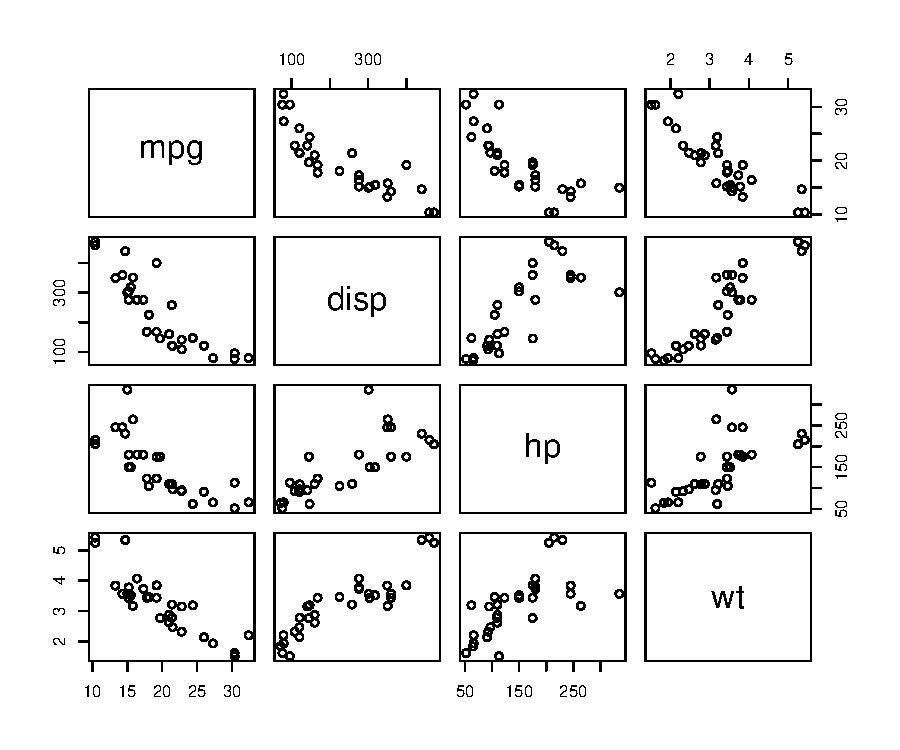
\includegraphics[width=.7\linewidth,height=.6\linewidth]{figure/unnamed-chunk-26-1} 

}



\end{knitrout}

\end{frame}

%------------------------------------------------

\begin{frame}[fragile]
\frametitle{High correlated variables}

\begin{knitrout}\footnotesize
\definecolor{shadecolor}{rgb}{0.969, 0.969, 0.969}\color{fgcolor}\begin{kframe}
\begin{alltt}
\hlcom{# matrix of correlations}
\hlkwd{cor}\hlstd{(df,} \hlkwc{use} \hlstd{=} \hlstr{'complete.obs'}\hlstd{)}
\end{alltt}
\begin{verbatim}
##             mpg       disp         hp         wt
## mpg   1.0000000 -0.8584325 -0.7729303 -0.8656222
## disp -0.8584325  1.0000000  0.7825073  0.8909678
## hp   -0.7729303  0.7825073  1.0000000  0.6386074
## wt   -0.8656222  0.8909678  0.6386074  1.0000000
\end{verbatim}
\end{kframe}
\end{knitrout}

\code{mpg} is most correlated with \code{wt}

\end{frame}

%------------------------------------------------

\begin{frame}[fragile]
\frametitle{Regression analysis with \code{lm()}}

\begin{knitrout}\scriptsize
\definecolor{shadecolor}{rgb}{0.969, 0.969, 0.969}\color{fgcolor}\begin{kframe}
\begin{alltt}
\hlcom{# matrix of correlations}
\hlstd{regression} \hlkwb{<-} \hlkwd{lm}\hlstd{(mpg} \hlopt{~} \hlstd{wt,} \hlkwc{data} \hlstd{= df)}

\hlkwd{summary}\hlstd{(regression)}
\end{alltt}
\begin{verbatim}
## 
## Call:
## lm(formula = mpg ~ wt, data = df)
## 
## Residuals:
##     Min      1Q  Median      3Q     Max 
## -4.3073 -2.0725 -0.2766  1.5742  7.4297 
## 
## Coefficients:
##             Estimate Std. Error t value Pr(>|t|)    
## (Intercept)   36.000      1.860  19.351  < 2e-16 ***
## wt            -5.013      0.548  -9.148 6.62e-10 ***
## ---
## Signif. codes:  0 '***' 0.001 '**' 0.01 '*' 0.05 '.' 0.1 ' ' 1
## 
## Residual standard error: 2.883 on 28 degrees of freedom
##   (2 observations deleted due to missingness)
## Multiple R-squared:  0.7493,	Adjusted R-squared:  0.7403 
## F-statistic: 83.69 on 1 and 28 DF,  p-value: 6.615e-10
\end{verbatim}
\end{kframe}
\end{knitrout}

\end{frame}

%------------------------------------------------

\begin{frame}[fragile]
\frametitle{Regression analysis with \code{lm()}}

\begin{knitrout}\footnotesize
\definecolor{shadecolor}{rgb}{0.969, 0.969, 0.969}\color{fgcolor}\begin{kframe}
\begin{alltt}
\hlcom{# prediction}
\hlkwd{predict}\hlstd{(regression,} \hlkwc{newdata} \hlstd{= df[}\hlkwd{c}\hlstd{(}\hlnum{5}\hlstd{,}\hlnum{20}\hlstd{),}\hlopt{-}\hlnum{1}\hlstd{])}
\end{alltt}
\begin{verbatim}
## Hornet Sportabout    Toyota Corolla 
##          18.75370          26.80021
\end{verbatim}
\begin{alltt}
\hlcom{# compare with true values}
\hlstd{mtcars}\hlopt{$}\hlstd{mpg[}\hlkwd{c}\hlstd{(}\hlnum{5}\hlstd{,}\hlnum{20}\hlstd{)]}
\end{alltt}
\begin{verbatim}
## [1] 18.7 33.9
\end{verbatim}
\end{kframe}
\end{knitrout}

\end{frame}

%------------------------------------------------

\begin{frame}
\begin{center}
\Huge{\hilit{Nearest Neighbors}}
\end{center}
\end{frame}

%------------------------------------------------

\begin{frame}
\frametitle{Imputation}

\bb{Imputing with similarities}
We can calculate distances or similarities between two or more observations
\eb

\end{frame}

%------------------------------------------------

\begin{frame}
\frametitle{Nearest Neighbors Idea}
\begin{center}
\ig[width=8cm]{images/knn1.pdf}
\end{center}
\end{frame}

%------------------------------------------------

\begin{frame}
\frametitle{Nearest Neighbors Idea}
\begin{center}
\ig[width=8cm]{images/knn2.pdf}
\end{center}
\end{frame}

%------------------------------------------------

\begin{frame}
\frametitle{Nearest Neighbors Idea}
\begin{center}
\ig[width=8cm]{images/knn3.pdf}
\end{center}
\end{frame}

%------------------------------------------------

\begin{frame}[fragile]
\frametitle{Nearest Neighbor Imputation}

\bbi
  \item observations near each other in $(u, v)$ space will have similar values (circles, crosses)
  \item find the $k=3$ nearest points in $(u, v)$ to the missing value
  \item let the circles and crosses vote
  \item if the neighbors have 2/3 circles or all circles, then assign circle, (cross otherwise)
\ei

\end{frame}

%------------------------------------------------

\begin{frame}
\frametitle{Nearest Neighbors Idea}
\begin{center}
\ig[width=8cm]{images/knn4.pdf}
\end{center}
\end{frame}

%------------------------------------------------

\begin{frame}
\frametitle{Nearest Neighbors Idea}
\begin{center}
\ig[width=8cm]{images/knn5.pdf}
\end{center}
\end{frame}

%------------------------------------------------

\begin{frame}[fragile]
\frametitle{Nearest Neighbor Imputation}

\bb{Questions}
\bbi
  \item How to choose $k$?
  \item How to choose $u, v, ...$? (predicting variables)
  \item What type of distance/similarity measure?
\ei
\eb

\end{frame}

%------------------------------------------------

\begin{frame}[fragile]
\frametitle{Nearest Neighbor Imputation}

Function {\hilit \code{knn()}} from package \code{"class"}
\begin{knitrout}\footnotesize
\definecolor{shadecolor}{rgb}{0.969, 0.969, 0.969}\color{fgcolor}\begin{kframe}
\begin{alltt}
\hlkwd{knn}\hlstd{(train, test, cl,} \hlkwc{k} \hlstd{=} \hlnum{1}\hlstd{,} \hlkwc{l} \hlstd{=} \hlnum{0}\hlstd{,} \hlkwc{use.all} \hlstd{=} \hlnum{TRUE}\hlstd{)}
\end{alltt}
\end{kframe}
\end{knitrout}

\bi
  \item \code{train} matrix or data frame of training set cases
  \item \code{test} matrix or data frame of test set cases
  \item \code{cl} factor of true classifications of training set
  \item \code{k} number of neighbors
\ei

\end{frame}

%------------------------------------------------

\begin{frame}[fragile]
\frametitle{Function \code{knn()}}

\begin{knitrout}\footnotesize
\definecolor{shadecolor}{rgb}{0.969, 0.969, 0.969}\color{fgcolor}\begin{kframe}
\begin{alltt}
\hlcom{# subset of 'mtcars'}
\hlstd{df} \hlkwb{<-} \hlstd{mtcars[ ,}\hlkwd{c}\hlstd{(}\hlstr{'mpg'}\hlstd{,} \hlstr{'disp'}\hlstd{,} \hlstr{'hp'}\hlstd{,} \hlstr{'wt'}\hlstd{)]}
\hlkwd{head}\hlstd{(df)}
\end{alltt}
\begin{verbatim}
##                    mpg disp  hp    wt
## Mazda RX4         21.0  160 110 2.620
## Mazda RX4 Wag     21.0  160 110 2.875
## Datsun 710        22.8  108  93 2.320
## Hornet 4 Drive    21.4  258 110 3.215
## Hornet Sportabout 18.7  360 175 3.440
## Valiant           18.1  225 105 3.460
\end{verbatim}
\end{kframe}
\end{knitrout}

\begin{knitrout}\footnotesize
\definecolor{shadecolor}{rgb}{0.969, 0.969, 0.969}\color{fgcolor}\begin{kframe}
\begin{alltt}
\hlcom{# missing values in 'mpg'}
\hlstd{df}\hlopt{$}\hlstd{mpg[}\hlkwd{c}\hlstd{(}\hlnum{5}\hlstd{,}\hlnum{20}\hlstd{)]} \hlkwb{<-} \hlnum{NA}
\hlstd{mpg} \hlkwb{<-} \hlstd{df}\hlopt{$}\hlstd{mpg}
\end{alltt}
\end{kframe}
\end{knitrout}

\end{frame}

%------------------------------------------------

\begin{frame}[fragile]
\frametitle{Function \code{knn()}}

\begin{knitrout}\footnotesize
\definecolor{shadecolor}{rgb}{0.969, 0.969, 0.969}\color{fgcolor}\begin{kframe}
\begin{alltt}
\hlkwd{library}\hlstd{(class)}

\hlstd{df_aux} \hlkwb{<-} \hlstd{df[ ,}\hlopt{-}\hlnum{1}\hlstd{]}               \hlcom{# data without mpg}
\hlstd{df_ok} \hlkwb{<-} \hlstd{df_aux[}\hlopt{!}\hlkwd{is.na}\hlstd{(mpg), ]}   \hlcom{# train set}
\hlstd{df_na} \hlkwb{<-} \hlstd{df_aux[}\hlkwd{is.na}\hlstd{(mpg), ]}    \hlcom{# test set}

\hlcom{# 1 nearest neighbor}
\hlstd{nn1} \hlkwb{<-} \hlkwd{knn}\hlstd{(}
  \hlkwc{train} \hlstd{= df_ok,}
  \hlkwc{test} \hlstd{= df_na,}
  \hlkwc{cl} \hlstd{= mpg[}\hlopt{!}\hlkwd{is.na}\hlstd{(mpg)],}
  \hlkwc{k} \hlstd{=} \hlnum{1}\hlstd{)}
\end{alltt}
\end{kframe}
\end{knitrout}

\end{frame}

%------------------------------------------------

\begin{frame}[fragile]
\frametitle{Function \code{knn()}}

\begin{knitrout}\footnotesize
\definecolor{shadecolor}{rgb}{0.969, 0.969, 0.969}\color{fgcolor}\begin{kframe}
\begin{alltt}
\hlcom{# imputed values}
\hlstd{nn1}
\end{alltt}
\begin{verbatim}
## [1] 19.2 32.4
## 23 Levels: 10.4 13.3 14.3 14.7 15 15.2 15.5 15.8 16.4 17.3 17.8 18.1 ... 32.4
\end{verbatim}
\begin{alltt}
\hlcom{# compared to real values}
\hlstd{mtcars}\hlopt{$}\hlstd{mpg[}\hlkwd{c}\hlstd{(}\hlnum{5}\hlstd{,}\hlnum{20}\hlstd{)]}
\end{alltt}
\begin{verbatim}
## [1] 18.7 33.9
\end{verbatim}
\end{kframe}
\end{knitrout}

\end{frame}

%------------------------------------------------

\begin{frame}[fragile]
\frametitle{Function \code{knn()}}

\begin{knitrout}\footnotesize
\definecolor{shadecolor}{rgb}{0.969, 0.969, 0.969}\color{fgcolor}\begin{kframe}
\begin{alltt}
\hlcom{# 3 nearest neighbor}
\hlstd{nn3} \hlkwb{<-} \hlkwd{knn}\hlstd{(}
  \hlkwc{train} \hlstd{= df_ok,}
  \hlkwc{test} \hlstd{= df_na,}
  \hlkwc{cl} \hlstd{= mpg[}\hlopt{!}\hlkwd{is.na}\hlstd{(mpg)],}
  \hlkwc{k} \hlstd{=} \hlnum{3}\hlstd{)}

\hlcom{# imputed values}
\hlstd{nn3}
\end{alltt}
\begin{verbatim}
## [1] 19.2 30.4
## 23 Levels: 10.4 13.3 14.3 14.7 15 15.2 15.5 15.8 16.4 17.3 17.8 18.1 ... 32.4
\end{verbatim}
\begin{alltt}
\hlcom{# real values}
\hlstd{mtcars}\hlopt{$}\hlstd{mpg[}\hlkwd{c}\hlstd{(}\hlnum{5}\hlstd{,}\hlnum{20}\hlstd{)]}
\end{alltt}
\begin{verbatim}
## [1] 18.7 33.9
\end{verbatim}
\end{kframe}
\end{knitrout}

\end{frame}

%------------------------------------------------

\begin{frame}
\begin{center}
\Huge{\hilit{R Packages \\ VIM and missMDA}}
\end{center}
\end{frame}

%------------------------------------------------

\begin{frame}[fragile]
\frametitle{Vim and missMDA}

\bi
  \item package \code{"VIM"} by Templ et al
  \item package \code{"missMDA"} by Francois Husson and Julie Josse
\ei
\begin{knitrout}\footnotesize
\definecolor{shadecolor}{rgb}{0.969, 0.969, 0.969}\color{fgcolor}\begin{kframe}
\begin{alltt}
\hlkwd{install.packacges}\hlstd{(}\hlkwd{c}\hlstd{(}\hlstr{"VIM"}\hlstd{,} \hlstr{"missMDA"}\hlstd{))}
\end{alltt}
\end{kframe}
\end{knitrout}

\begin{knitrout}\footnotesize
\definecolor{shadecolor}{rgb}{0.969, 0.969, 0.969}\color{fgcolor}\begin{kframe}
\begin{alltt}
\hlkwd{library}\hlstd{(VIM)}
\end{alltt}


{\ttfamily\noindent\bfseries\color{errorcolor}{\#\# Error in library(VIM): there is no package called 'VIM'}}\begin{alltt}
\hlkwd{library}\hlstd{(missMDA)}
\end{alltt}


{\ttfamily\noindent\bfseries\color{errorcolor}{\#\# Error in library(missMDA): there is no package called 'missMDA'}}\end{kframe}
\end{knitrout}

\end{frame}

%------------------------------------------------

\begin{frame}[fragile]
\frametitle{Data \code{ozone}}

Data \code{ozone} (in \code{"missMDA"}): daily measurements of meteorological variables and ozone concentration:
\begin{knitrout}\tiny
\definecolor{shadecolor}{rgb}{0.969, 0.969, 0.969}\color{fgcolor}\begin{kframe}
\begin{alltt}
\hlkwd{data}\hlstd{(ozone)}
\end{alltt}


{\ttfamily\noindent\color{warningcolor}{\#\# Warning in data(ozone): data set 'ozone' not found}}\begin{alltt}
\hlkwd{head}\hlstd{(ozone,} \hlkwc{n} \hlstd{=} \hlnum{5}\hlstd{)}
\end{alltt}


{\ttfamily\noindent\bfseries\color{errorcolor}{\#\# Error in head(ozone, n = 5): object 'ozone' not found}}\end{kframe}
\end{knitrout}

\end{frame}

%------------------------------------------------

\begin{frame}[fragile]
\frametitle{Data \code{ozone}}

Number of missing values in each variable:
\begin{knitrout}\footnotesize
\definecolor{shadecolor}{rgb}{0.969, 0.969, 0.969}\color{fgcolor}\begin{kframe}
\begin{alltt}
\hlstd{num_na} \hlkwb{<-} \hlkwd{sapply}\hlstd{(ozone,} \hlkwa{function}\hlstd{(}\hlkwc{x}\hlstd{)} \hlkwd{sum}\hlstd{(}\hlkwd{is.na}\hlstd{(x)))}
\end{alltt}


{\ttfamily\noindent\bfseries\color{errorcolor}{\#\# Error in lapply(X = X, FUN = FUN, ...): object 'ozone' not found}}\begin{alltt}
\hlstd{num_na[}\hlnum{1}\hlopt{:}\hlnum{7}\hlstd{]; num_na[}\hlnum{8}\hlopt{:}\hlnum{13}\hlstd{]}
\end{alltt}


{\ttfamily\noindent\bfseries\color{errorcolor}{\#\# Error in eval(expr, envir, enclos): object 'num\_na' not found}}

{\ttfamily\noindent\bfseries\color{errorcolor}{\#\# Error in eval(expr, envir, enclos): object 'num\_na' not found}}\end{kframe}
\end{knitrout}

\end{frame}

%------------------------------------------------

\begin{frame}[fragile]
\frametitle{Looking at missing values}

\begin{knitrout}\footnotesize
\definecolor{shadecolor}{rgb}{0.969, 0.969, 0.969}\color{fgcolor}\begin{kframe}
\begin{alltt}
\hlcom{# aggregation for missing values}
\hlstd{oz_aggr} \hlkwb{<-} \hlkwd{aggr}\hlstd{(ozone,} \hlkwc{prop} \hlstd{=} \hlnum{TRUE}\hlstd{,}
       \hlkwc{combined} \hlstd{=} \hlnum{TRUE}\hlstd{,} \hlkwc{plot} \hlstd{=} \hlnum{FALSE}\hlstd{)}
\end{alltt}


{\ttfamily\noindent\bfseries\color{errorcolor}{\#\# Error in eval(expr, envir, enclos): could not find function "{}aggr"{}}}\begin{alltt}
\hlcom{# summary}
\hlstd{res} \hlkwb{<-} \hlkwd{summary}\hlstd{(oz_aggr)}
\end{alltt}


{\ttfamily\noindent\bfseries\color{errorcolor}{\#\# Error in summary(oz\_aggr): error in evaluating the argument 'object' in selecting a method for function 'summary': Error: object 'oz\_aggr' not found}}\end{kframe}
\end{knitrout}

\end{frame}

%------------------------------------------------

\begin{frame}[fragile]
\frametitle{Looking at missing values}

\begin{knitrout}\footnotesize
\definecolor{shadecolor}{rgb}{0.969, 0.969, 0.969}\color{fgcolor}\begin{kframe}
\begin{alltt}
\hlcom{# variables sorted by number of missings}
\hlstd{res}\hlopt{$}\hlstd{missings[}\hlkwd{order}\hlstd{(res}\hlopt{$}\hlstd{missings[,}\hlnum{2}\hlstd{]), ]}
\end{alltt}


{\ttfamily\noindent\bfseries\color{errorcolor}{\#\# Error in eval(expr, envir, enclos): object 'res' not found}}\end{kframe}
\end{knitrout}

\end{frame}

%------------------------------------------------

\begin{frame}[fragile]
\frametitle{Looking at missing values}

\begin{knitrout}\footnotesize
\definecolor{shadecolor}{rgb}{0.969, 0.969, 0.969}\color{fgcolor}\begin{kframe}
\begin{alltt}
\hlcom{# combinations}
\hlkwd{head}\hlstd{(res}\hlopt{$}\hlstd{combinations,} \hlkwc{n} \hlstd{=} \hlnum{10}\hlstd{)}
\end{alltt}


{\ttfamily\noindent\bfseries\color{errorcolor}{\#\# Error in head(res\$combinations, n = 10): object 'res' not found}}\end{kframe}
\end{knitrout}

\end{frame}

%------------------------------------------------

\begin{frame}[fragile]
\frametitle{Looking at missing values}

\begin{knitrout}\footnotesize
\definecolor{shadecolor}{rgb}{0.969, 0.969, 0.969}\color{fgcolor}\begin{kframe}
\begin{alltt}
\hlcom{# combinations}
\hlkwd{tail}\hlstd{(res}\hlopt{$}\hlstd{combinations,} \hlkwc{n} \hlstd{=} \hlnum{10}\hlstd{)}
\end{alltt}


{\ttfamily\noindent\bfseries\color{errorcolor}{\#\# Error in tail(res\$combinations, n = 10): object 'res' not found}}\end{kframe}
\end{knitrout}

\end{frame}

%------------------------------------------------

\begin{frame}[fragile]
\frametitle{Looking at missing values}

\begin{knitrout}\footnotesize
\definecolor{shadecolor}{rgb}{0.969, 0.969, 0.969}\color{fgcolor}\begin{kframe}
\begin{alltt}
\hlcom{# visualizations}
\hlkwd{plot}\hlstd{(oz_aggr)}
\end{alltt}


{\ttfamily\noindent\bfseries\color{errorcolor}{\#\# Error in plot(oz\_aggr): error in evaluating the argument 'x' in selecting a method for function 'plot': Error: object 'oz\_aggr' not found}}\end{kframe}
\end{knitrout}

\end{frame}

%------------------------------------------------

\begin{frame}[fragile]
\frametitle{Looking at missing values}

\begin{knitrout}\footnotesize
\definecolor{shadecolor}{rgb}{0.969, 0.969, 0.969}\color{fgcolor}\begin{kframe}
\begin{alltt}
\hlcom{# visualizations}
\hlkwd{matrixplot}\hlstd{(ozone,} \hlkwc{sortby} \hlstd{=} \hlnum{2}\hlstd{)}
\end{alltt}


{\ttfamily\noindent\bfseries\color{errorcolor}{\#\# Error in eval(expr, envir, enclos): could not find function "{}matrixplot"{}}}\end{kframe}
\end{knitrout}

\end{frame}

%------------------------------------------------

\begin{frame}[fragile]
\frametitle{Looking at missing values}

\begin{knitrout}\footnotesize
\definecolor{shadecolor}{rgb}{0.969, 0.969, 0.969}\color{fgcolor}\begin{kframe}
\begin{alltt}
\hlcom{# visualizations}
\hlkwd{marginplot}\hlstd{(ozone[ ,}\hlkwd{c}\hlstd{(}\hlstr{'T9'}\hlstd{,} \hlstr{'maxO3'}\hlstd{)])}
\end{alltt}


{\ttfamily\noindent\bfseries\color{errorcolor}{\#\# Error in eval(expr, envir, enclos): could not find function "{}marginplot"{}}}\end{kframe}
\end{knitrout}

\end{frame}

%------------------------------------------------

\begin{frame}
\frametitle{More info ...}

\bi
  \item Is there a pattern of missing values?
  \item Is there a mechanism leading to missing values?
  \bi
    \item purely random?
    \item probability model for missing values?
  \ei
  \item There are more sophisticated options: \\
  ``Missing Data: Our View of the State of the Art'' (Schafer \& Graham, 2000)
  \item Bayesian imputation
  \item Multiple imputation
  \item \textit{etc}
\ei

\end{frame}

%------------------------------------------------

\end{document}
